%----------------------------------------------------------------------------
\chapter{Overview of the Approach}
%----------------------------------------------------------------------------
In this chapter, the various aspects of the proposed approach are detailed. In Section \ref{sec_methodology}, the application of this methodology from the users' point of view: how are they supposed to interact with the interactive automata learning framework and how can they utilize it to design reactive systems in a declarative way. Then, in Section \ref{sec_architecture}, the applied software architecture, software components, algorithms and data structures are presented in the following order: first, the components concerned with the automata learning algorithm, then those responsible for its interaction with the oracle, then the possible interactions of the oracle with the engineer.
%----------------------------------------------------------------------------
\section{Overview of the Methodology} \label{sec_methodology}
%----------------------------------------------------------------------------
\begin{figure}[!ht] 
	\centering
	\fbox{
		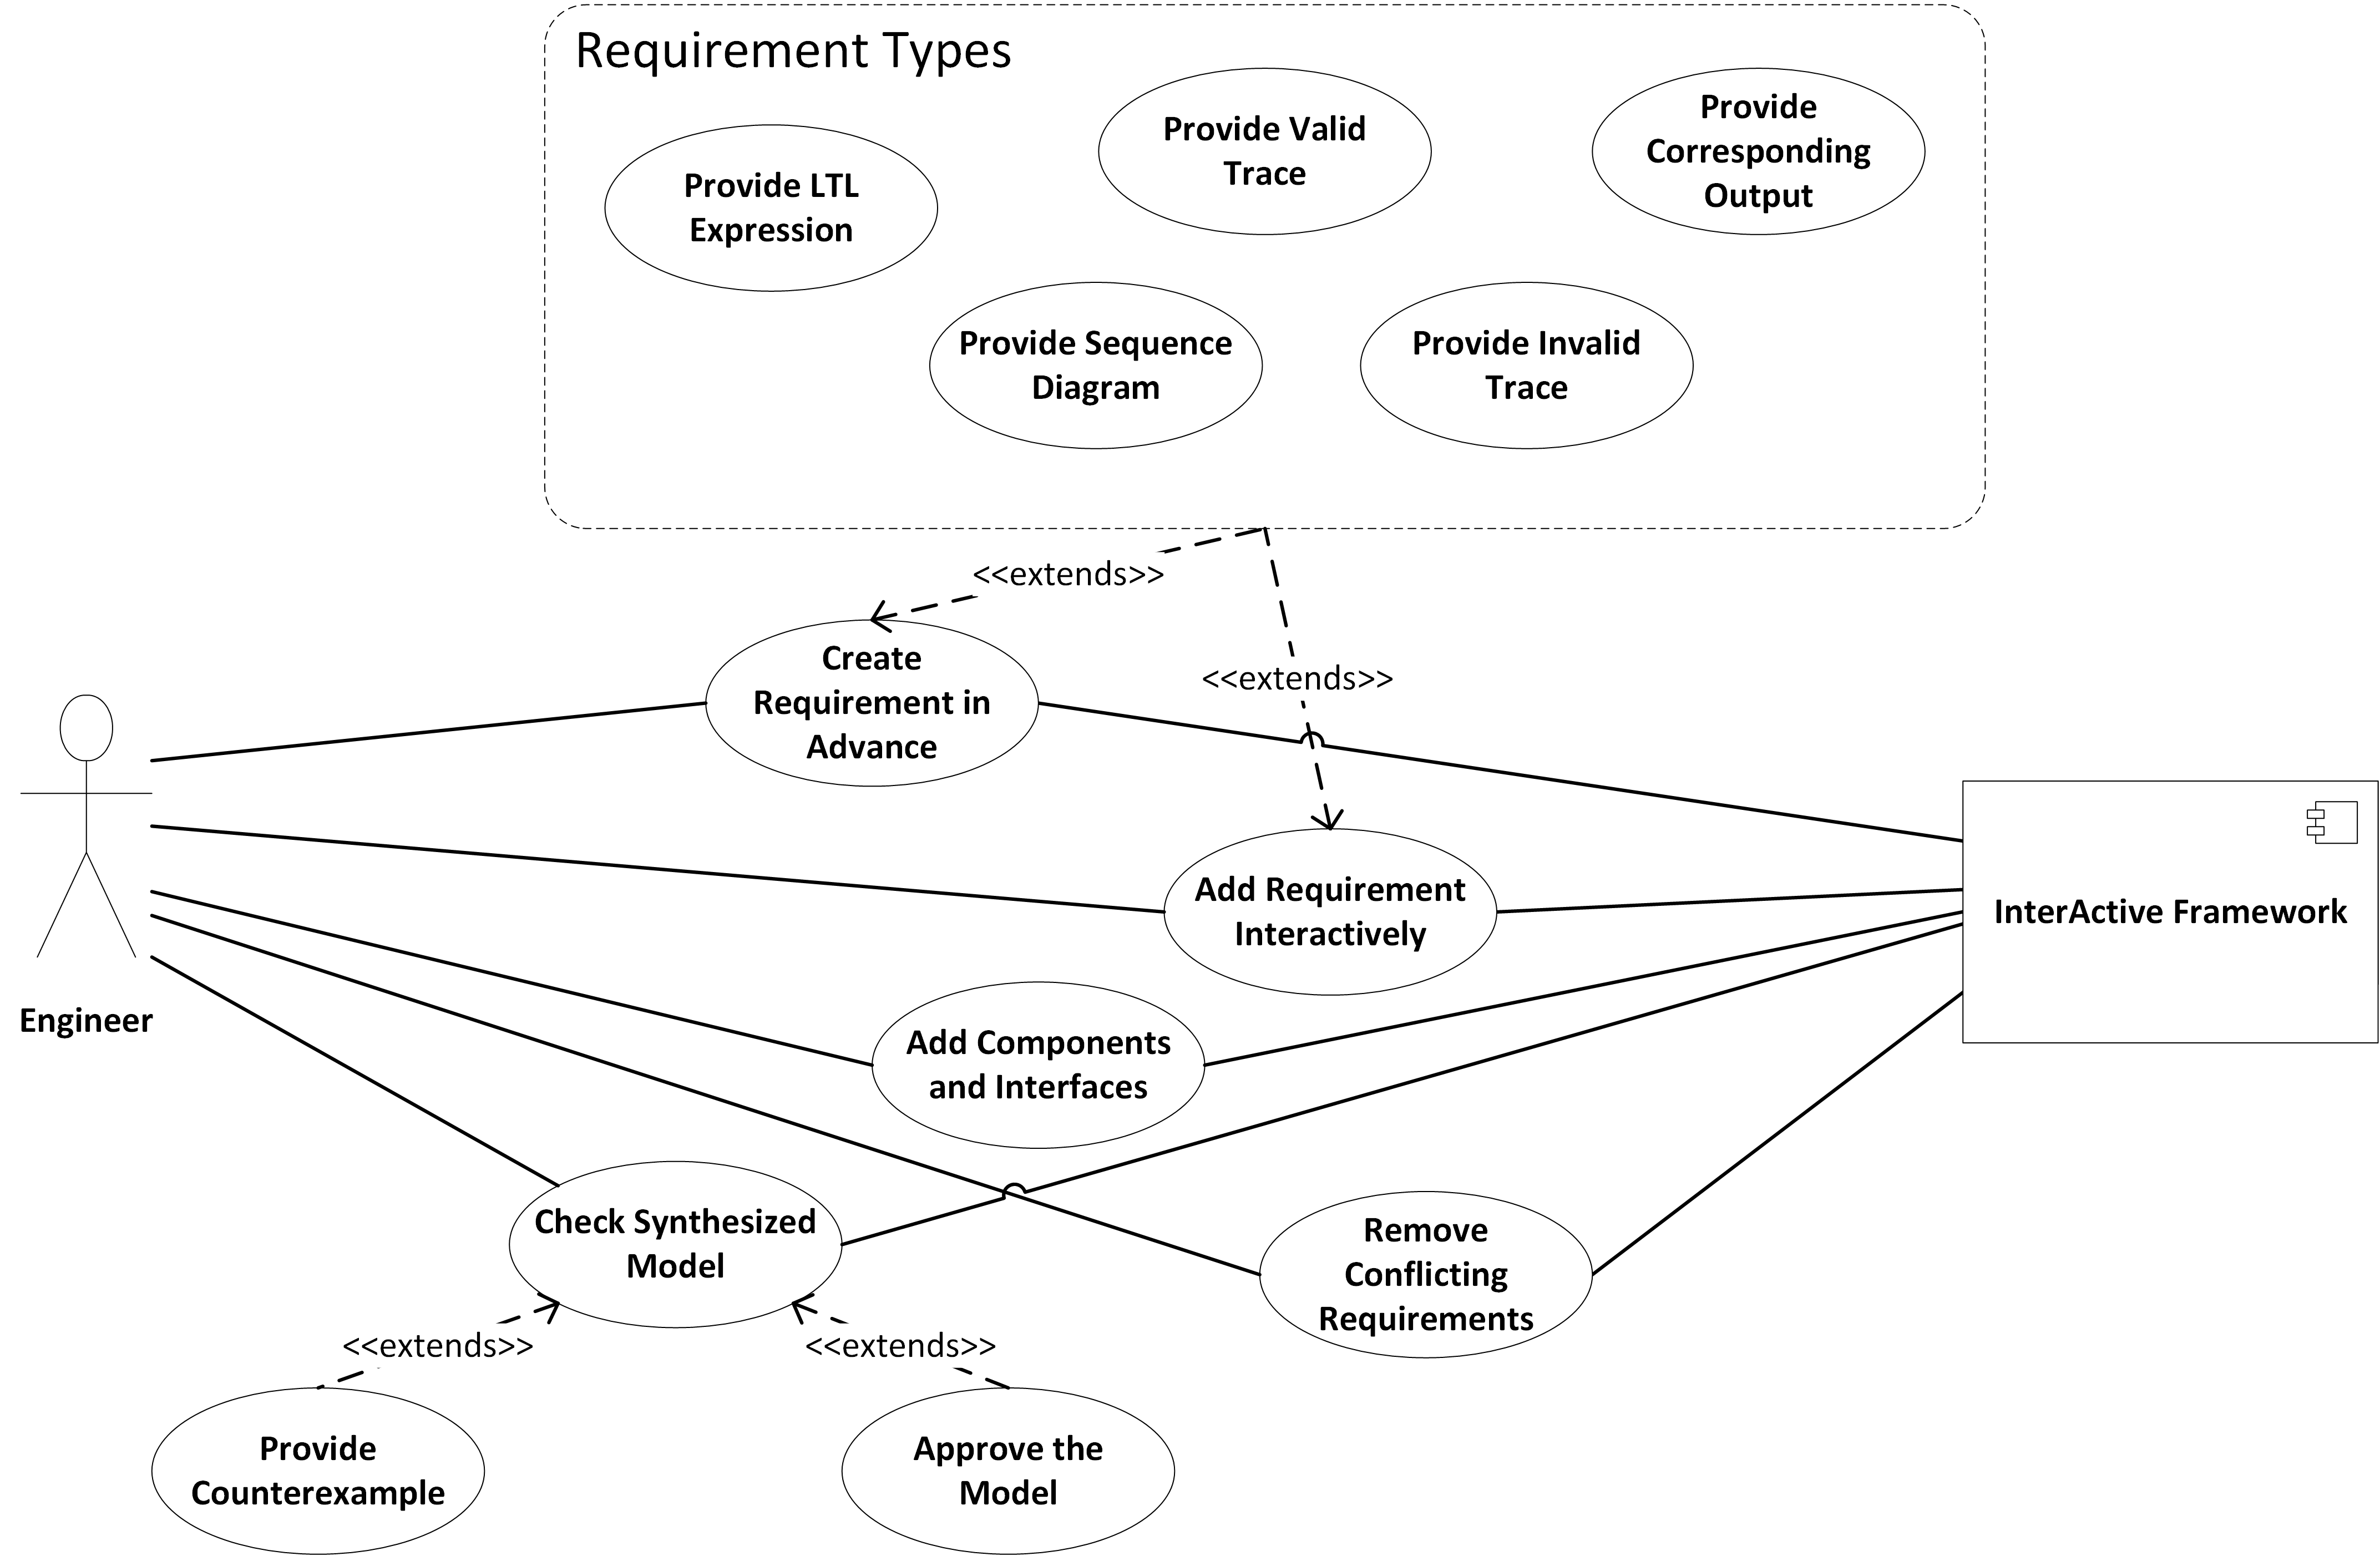
\includegraphics[width=150mm, keepaspectratio]{figures/methodology_interactiontypes.png}
	}
	\caption{Possibilities of the Engineer} %TODO title 
	\label{fig_methodology_interactiontypes}
\end{figure}

Our methodology is heavily based on the interaction of the user with the system, especially its \textit{Oracle} component. The different types of interaciton are summarized on Figure \ref{fig_methodology_interactiontypes} and elaborated on in Subsection \ref{subs_reqtypes}. These interactions take place in a predefined order - the \textit{proposed workflow}, illustrated on Figure \ref{fig_methodology_workflow}. This workflow consists of two phases: first, an \textit{offline} one, and then an \textit{online} one. During the offline phase, the system offers little assistance, the designing engineer must determine the required details by other means. The interactive system design happens during the online phase. 

The individual steps in both the offline and the online phases have a predefined syntax with the corresponding, precisely defined semantics. Their common feature is the declarative way of describing the system components, which allows the engineer to focus solely on the expected behavior and acquire a minimal model exhibiting the specified functionality. The following subsections explain these steps in detail.

\begin{figure}[!ht] 
	\centering
	\fbox{
		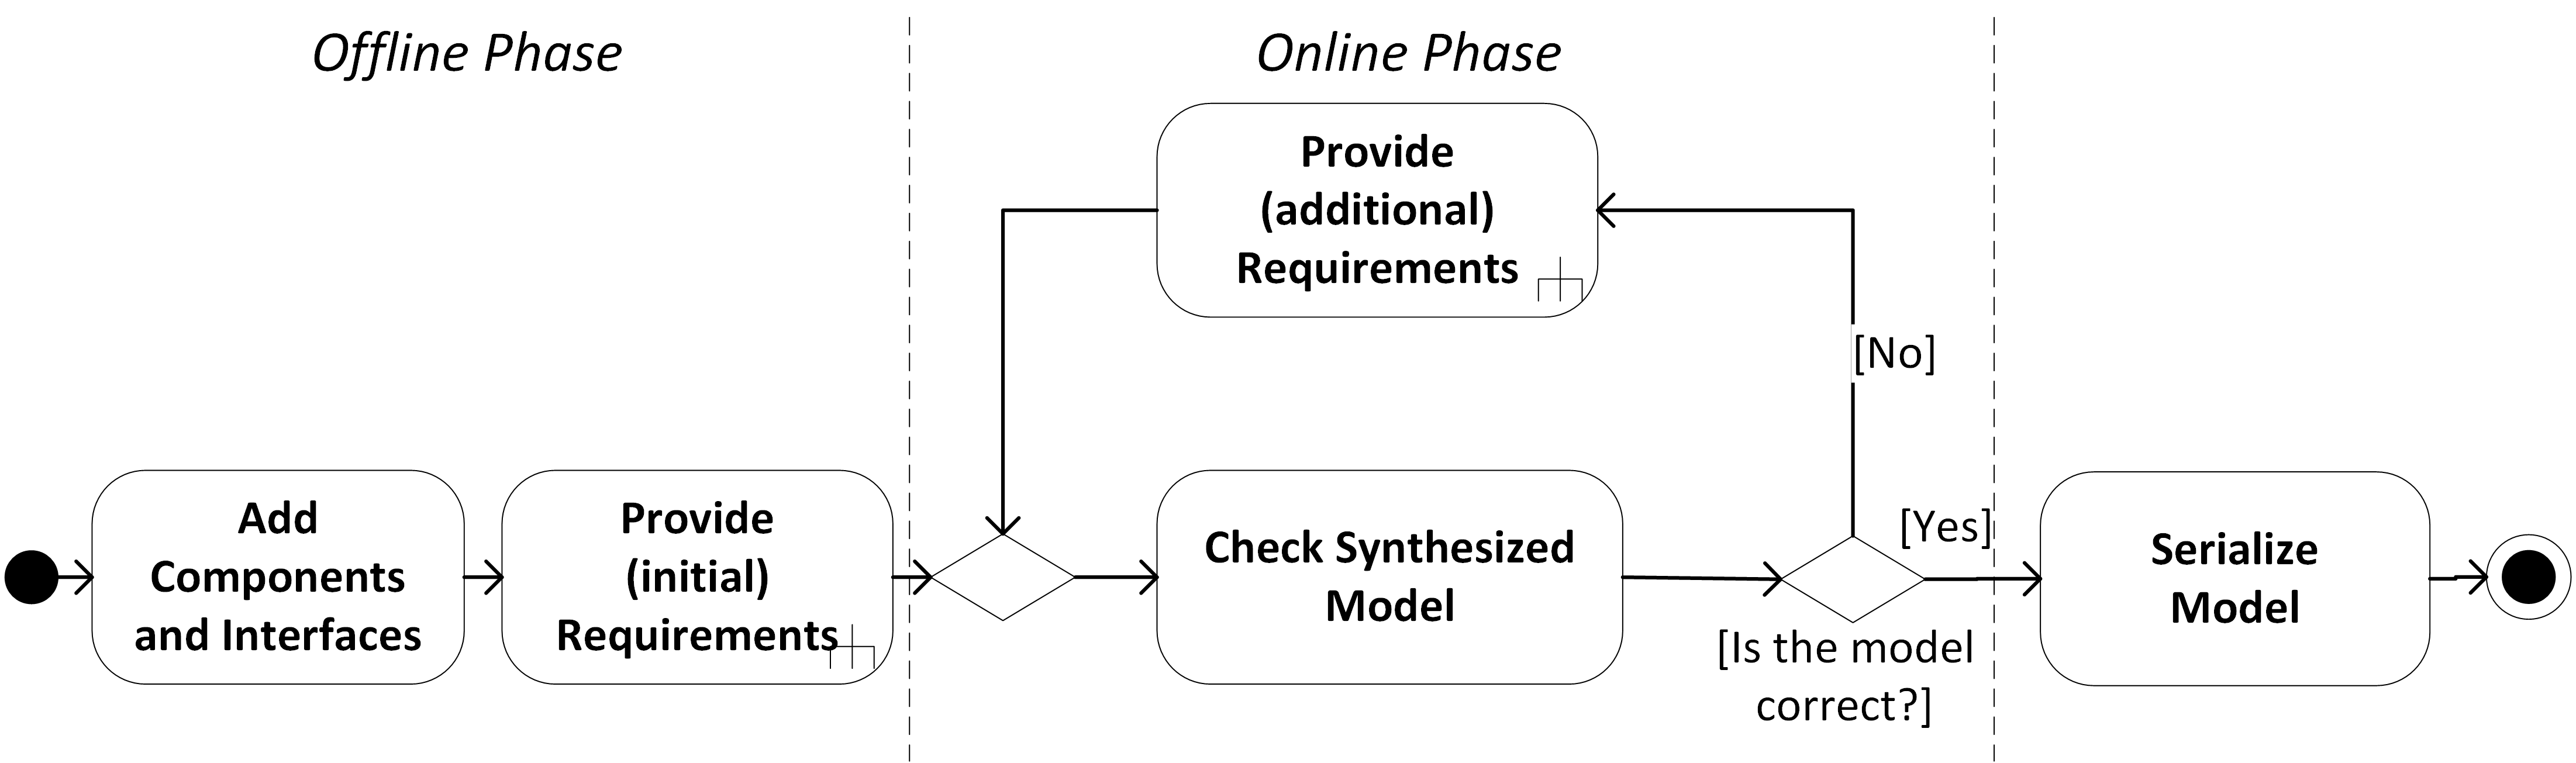
\includegraphics[width=150mm, keepaspectratio]{figures/methodology_workflow.png}
	}
	\caption{The Proposed Workflow} %TODO title 
	\label{fig_methodology_workflow}
\end{figure}
%TODO fork a komponenseknek
%TODO bekeretezni az online és az offline részeket, meg feliratozni

%---------------------------------------------------------------
\subsection{Component and Interface Definition} \label{subs_compdef}
%---------------------------------------------------------------
%TODO megadhat több komponenst, névvel, ezek a megfelelő viselkedéseket fogják tanúsítani. I/O ábécét megadjuk előre, komponensek kapcsolatát a nevekből inferáljuk. Mindegyiket TELJESEN KÜLÖN tanuljuk (fork). Ezért egyelőre semmit sem garantálunk ilyen téren.
The first step of the workflow is the declaration of the system components. This happens in the offline phase, as the determination of the system components, their exact boundaries and interfaces is out of the scope of this work. Nonetheless, the engineer must provide the names of the system components, along with their input- and output alphabets, before the workflow can proceed to the next step.

Users are encouraged to specify input and output characters qualified with port names in the format 'Port.character', as this supplies the subsequent steps with essential information about the connections of the individual system components.

The components are handled as independent systems in every other aspect. This results - among others - in the arbitrary ordering of the online behavior-learning phases, and the behavioral faults being limited to their components of origin (although this does not limit the propagation of errors through messages resulting from incorrect behavior).

The syntax of component and interface definitions is quite simple, as illustrated in [TODO add example]

%---------------------------------------------------------------
\subsection{Requirement Types} \label{subs_reqtypes}
%---------------------------------------------------------------
%TODO kifejteni minden típust egyesével (5).
% Trace-based vagy program logic (def ref background)
% Mi a szintaxis (LTL: syntactic constructs, operátor precedencia, szemandtika - hivatkozások a megfelelő cikkre)
% Mi a szemantika (LTL->LTS alapú def ref background)
%---------------------------------------------------------------
\subsection{Conflicting Requirements} \label{subs_conf}
%---------------------------------------------------------------
%TODO konfliktusban álló követelményeket mikor tud kivenni
% Diszjunktság nehéz kérdés (ref Backgr), csak akkor dobjuk fel, ha valami bemenetre gond van
% Akkor kiveheti az egyiket
% Konzisztenciát többé-kevésbé figyeljük

%---------------------------------------------------------------
\subsection{Equivalence Query} \label{subs_eq}
%---------------------------------------------------------------
%TODO megjeleníti az EQt, mi van ekkor
% Ha tetszik, elfogadjuk és továbblép a workflowban
% Ha nem tetszik, adunk egy ellenpélda-input-sorozatot
% TULAJDONSÁGAI?
%---------------------------------------------------------------
\subsection{The Resulting Model} \label{subs_resultingmodel}
%---------------------------------------------------------------
%TODO ha minden kész, valid Gammát kapunk, ezt:
% kiegészíthetjük
% generálhatunk belőle akármit, amit a gamma tud (ref backgr)

%----------------------------------------------------------------------------
\section{Overview of the Architecture} \label{sec_architecture}
%----------------------------------------------------------------------------